\documentclass[11pt,a4paper]{article}
\usepackage[utf8]{inputenc}
\usepackage[slovak]{babel}
\usepackage[IL2]{fontenc}
\usepackage{amsmath}
\usepackage{amsfonts}
\usepackage{cite}
\usepackage{amssymb}
\usepackage{alltt}
\usepackage{graphicx}
\usepackage[left=2cm,right=2cm,top=2cm,bottom=2cm]{geometry}
\author{Matúš Kontra}
\title{Dokumentácia Projektu Predmetu Soft Computing}
\author{Matúš Kontra}
\begin{document}

\begin{titlepage}
\begin{center}
{\textsc{Vysoké učení technické v Brně}}\\
{\textsc{Fakulta informačních technologií}}\\
\includegraphics[width=0.5\textwidth]{fit_logo.eps} \\
\Large{\textup{Projekt Predmetu Soft Computing\\}}
\Huge{\textup{Učenie neurónovej siete algoritmom simulovaného žíhania}}
\vspace{\stretch{0.618}}
\end{center}
{ \today \hfill
Matúš Kontra (xkontr00@stud.fit.vutbr.cz)}
\end{titlepage}

\tableofcontents
\newpage
\section{Úvod}
Projekt sa venoval implementácii doprednej neurónovej siete a dvom principiálne odlišným spôsobom jej učenia. Jedným z nich bol postup známi pod menom Backpropagation - technika založená na gradientoch, zmene váh takým smerom, ktorý spôsobí zníženie chyby. Toto má však neblahý následok spôsobujúci uviaznutie hľadania v lokálnych extrémoch. Preto som sa rozhodol otestovať učenie globálnou optimalizačnou metódou zvanou simulované žíhanie, ktorá je konštruovaná tak, aby bolo možné zabrániť vzniku tejto situácie.
\section{Teoretické podklady}
\subsection{Dopredná viacvrstvová neurónová sieť}
Neurónová sieť je koncept inšpirovaný nervovým systémom živých tvorov. Jej základným prvkom je perceptron - umelé napodobnenie a zabstrahovanie biologického neurónu. Neurón pozostáva z dendritov ( vstupy ), tela, a axónu (výstup). Hodnota výstupu neurónu je závislá na jeho vstupoch a ich hodnotách. Pri implementácii umelého neurónu existuje viacero možností ako s týmito vstupmi pracovať. Pre nás bude však nutné vedieť, že výstup závisí na sume vstupov vynásobených váhami, ktorá je použitá ako argument aktivačnej funkcie ( lineárna, sigmoidálna ). Táto udáva výstup neurónu.\\
Kľúčové pre použite neurónu je možnosť meniť váhy vstupov - hľadanie vhodných váh pre neurón nazývame učenie neurónu. Existujue mnoho postupov, ako biológiou inšpirovaných tak aj čisto teoretických, ktoré možno použiť. Platí, že žiaden z možných algoritmov není vhodný pre každý jeden problém.\\
\begin{center}
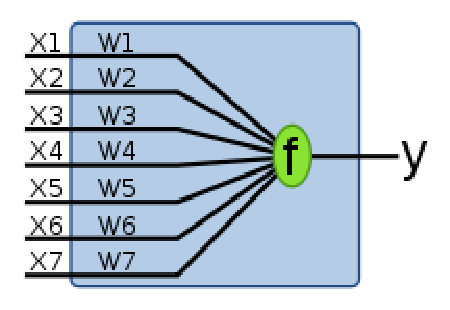
\includegraphics[scale=0.7]{200px-Perceptron.svg.eps.ps}\\
{\small $w_i$ sú váhy, f je aktivačná funkcia}  
\end{center}
Neurónovou sieťou nazývame štruktúru, vznikajúcu poprepájaním množiny neurónov. 
Sieť, v ktorej platí, že neuróny sú usporiadané do vrstiev ( vstupná, skrytá, výstupná ) a výstupy neurónu vrstvy predchádzajúcej vstupujú na vstupy vrstvy nasledujúcej a nikam inam, nazývame doprednou neurónovou sieťou. Ak je počet vrstiev neurónov vyšší ako jeden, nazveme sieť viacvrstvý perceptron.\\
\begin{center}
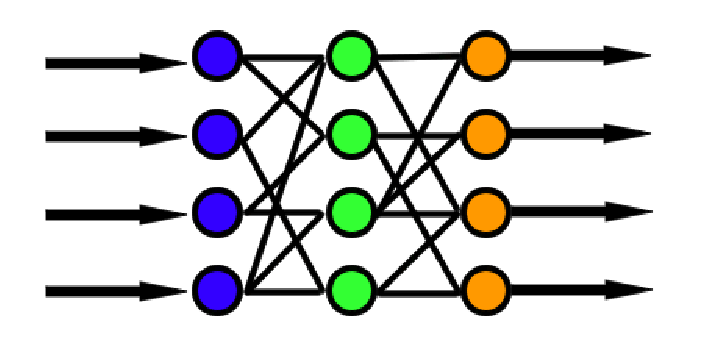
\includegraphics[scale=0.7]{ffn.ps}\\
\end{center}
Ďalej treba poznamenať, že je možné používať rôzne spôsoby výpočtu vnútorného potenciálu, ako aj rozmanité aktivačné funkcie. V tomto projekte budeme pracovať s perceptronmi používajúcimi lineárnu bázovú funkciu a sigmoidálnu aktivačnú funkciu (hyperbolický tangens).
\subsection{Učenie neurónovej siete}
\subsubsection{Backpropagation}
Jedna z najčastejšie používaných metód pre učenie neurónových sietí. Jedná sa o metódu učenia s učiteľom - máme k dispozícii páry vektorov udávajúce očakávaný výstup pre istý vstup. \\
Principiálne sa jedná o metódy, počítajúcu gradient chyby vzhľadom na váhy siete a na jeho základe ich upravujú tak aby došlo k zníženiu celkovej chyby. Tento algoritmus má výhodu v tom, že veľmi rýchlo konverguje k vhodným lokálnym minimám.\\
Postup učenia je približne nasledujúci: Pre zvolený vzorok vypočítame odozvu siete a chybu s ktorou bol klasifikovaný. Na základe tejto chybu určíme deltu výstupnej vrstvy ( závislá na tvare aktivačnej funkcie, počíta sa na základe jej derivácie ). Deltu skrytých vrstiev počítame na základe výstupnej vrstvy a následné skryté vrstvy vzhľadom k váham. Po tom čo sme vypočítali všetky možné delty prechádzame sieťou od vstupnej vrstve k výstupnej. A na základe vstupov, délt a koeficientov učenia modifikujeme váhy.\\
Ako bolo popísané metóda konverguje rýchlo, avšak nie je schopná uniknúť lokálnym extrémom. Tomuto sa budeme pokúšať vyhnúť použitím algoritmu simulovaného žíhania.
\subsubsection{Simulované žíhanie}
Jedná sa o globálny optimalizačný algoritmus, inšpirovaný metalurgiou a procesom, ktorý nastáva pri ochladzovaní vysokozahriateho kovu, kým nenabudne pevného skupenstva. Únik z lokálnych miním je možný vďaka možnosti prejsť do menej dobrého stavu s istou pravdepodobnosťou.\\
Majme funkciu \textit{f(X)}, ktorú chceme minimalizovať, v našom prípade je to chyba siete a X je vektor váh. Ďalej potrebujeme $T_{poc}$, $T_{konc}$, funkciu výpočtu nového stavu, a funkciu výpočtu pravdepodobnosti prijatia nového stavu. Naša implementácia pracuje v dvoch zanorených cykloch, vonkajší riadi pokles teploty, vo vnútornom prebehne cyklus chladenia istý počet krát pri jednej teplote a do ďalšieho vonkajšieho cyklu prechádza najlepšie riešenie. Funkcia následujúceho stavu berie ako parameter teplotu a na jej základe modifikuje vektor váh - čím nižšia teplota, tým nižší rozptyl. Funkcia pravdepodobnosti nasledujúceho stavu vracia pravdepodobnosť 1.0 pre stav s nižšiou energiou. Pre stav s vyššou energiou berie do úvahy celkovú chybu, odchýlku od súčasného stavu a súčasnú teplotu a vracia pravdepodobnosť menšiu ako 1.0 primárne závislú na teplote.\cite{sabp}\cite{heaton}
\begin{alltt}
Anneal:
\hspace*{10mm} current = generuj_nový_stav()
\hspace*{10mm} best = current
\hspace*{10mm} t = tmax
\hspace*{10mm} pokiaľ t < tmin:
\hspace*{20mm} opakuj n krát - kde n je špecifikovaný počet opakovaní na jednej teplotnej úrovni:
\hspace*{30mm} next = generuj_nový_stav()
\hspace*{30mm} Ak uniform(0,1) < P(next, current, t):
\hspace*{40mm} current = next
\hspace*{40mm} Ak E(current) < E(next):
\hspace*{50mm} best = current
\hspace*{20mm} zníž teplotu t 
\hspace*{10mm} vráť best 
\end{alltt} 
\newpage
\section{Implementácia}
Implementačný jazyk bol zvolený Python 2.7. Extenzívne je využívaná knižnica numpy - na efektívne numerické výpočty nad n-rozmernými poliami.
\subsection{Neurónová sieť}
Sieť je objekt, zahrňujúci maticu váh pre každú skrytú a výstupnú vrstvu ( zoznam, dĺžka závislá na počte vrstiev ). Pre výstupy jednotlivých vrstiev máme vektory. Matice váh obsahujú aj stĺpec pre váhy bias neurónu. Výpočet výstupu vrstvy je riešený ako skalárny súčin matice váh a vektora výstupov vrstvy predchádzajúcej, resp. vstupu. 
\begin{alltt}
\begin{small}
self.HidWeights = []
self.HidWeights.append(((numpy.random.rand(Hid[0], self.In + 1)-1)*0.4)) \#matica vstupov na skrytú vrstvu
\# matice naviazania skrytých vrstiev
self.HidWeights.extend([((numpy.random.rand(Hid[i], Hid[i-1] + 1)-1)*0.4) for i in range(1,len(Hid))]) 

\# posledná skrytá na výstupnú
self.OutWeights = ((numpy.random.rand(Out, Hid[-1] + 1)-1)*1)
\end{small}
\end{alltt}
Z kódu možno vidieť, že váhy sú inicializované z intervalu (-0.4, 0.4 )\\
Výpočet neurónovej siete:
\begin{alltt}
\#prvá skrytá
numpy.dot(self.HidWeights[0], self.InActvs, out=self.HidActvs[0][0:-1])
numpy.tanh(self.HidActvs[0][0:-1], out=self.HidActvs[0][0:-1])

\#skryté
for i in range(1, len(self.HidWeights)):
	numpy.dot(self.HidWeights[i],self.HidActvs[i-1], out=self.HidActvs[i][0:-1])
	numpy.tanh(self.HidActvs[i][0:-1], out=self.HidActvs[i][0:-1])
	
\#výstupná -- OutActvs je výstup neurónovej siete
numpy.dot(self.OutWeights, self.HidActvs[-1], out=self.OutActvs)
numpy.tanh(self.OutActvs, out=self.OutActvs)
\end{alltt}
Funkcia numpy.dot vypočíta skalárny súčin matice a vektora a uloží ho do vektora výstupov, na ktorý je potom aplikovaná aktivačná funkcia numpy.tanh (po prvkoch vektora, ukladáme do toho istého vektora).\\

\subsection{Backpropagation trainer}
Konštruovaný nad sieťou, spolu s parametrom učenia. Učenie sa spúšťa metódou \texttt{train} parametrizovanou 
trénovacou množinou a špecifikáciou chyby a maximálneho počtu iterácii. Táto metóda pracuje v dvoch cykloch - vonkajší prechádza špecifikovaným rozsahom iterácii a vnútorna volá pre každú položku trénovacej množiny metódu \texttt{backpropagate} a počíta sumu štvorcov chyby pre trénovaciu množinu. Končí ak je chyba menšia ako bolo špecifikované, alebo bol vyčerpaný počet iterácii.\\
Metóda backpropagate vypočíta chybu pre zvolený prvok trénovacej množiny a upraví váhy neurónovej siete.
Najskôr sa vypočíta vektor chýb výstupnej vrstvy ako rozdiel očakávaného výstupu a skutočného výstupu siete. Táto hodnota slúži ako základ výpočtu delty neurónov výstupnej vrstvy. Výpočet délt sa propaguje smerom dozadu ( back-propagation ). Delta predchádzajúcej vrstvy sa vypočíta na základe váh, ktoré majú prepojenia na neuróny vrstvy nasledujúcej a ich delty. Na toto sa opäť používajú maticové operácie, konkrétne transponovaná matica váh a vektor délt.
\begin{alltt}
\begin{small}
\#delty výstupnej vrstvy
self.odelta = (1.0 - (self.net.OutActvs*self.net.OutActvs))*(expectedValues - self.net.OutActvs)
\#delty poslednej skrytej vrstvy
self.hdelta[-1] = (1.0-(self.net.HidActvs[-1]*self.net.HidActvs[-1]))*(dot(numpy.transpose(self.net.OutWeights),self.odelta) )
\#delty skrytých vrstiev
for i in reversed(xrange(len(self.net.HidWeights) - 1)):
	self.hdelta[i] = (1.0 - (self.net.HidActvs[i]*self.net.HidActvs[i]))*( dot(numpy.transpose(self.net.HidWeights[i]),self.hdelta[i+1][0:-1]) )
\end{small}
\end{alltt}
numpy.transpose transponuje maticu, numpy.dot vypočíta skalárny súčin a výraz
\texttt{(1.0 - (self.net.HidActvs[i]*self.net.HidActvs[i])) } reprezentuje deriváciu aktivačnej funkcie.\\
Po výpočte délt upravujeme váhy siete, na základe délt, hodnôt vstupov a parameru učenia.
\begin{alltt}
\begin{small}
for i in range(len(self.net.HidWeights[0])):
	numpy.add(self.net.HidWeights[0][i], (self.N*self.net.InActvs*self.hdelta[0][i]), out = self.net.HidWeights[0][i])

for i in range(1, len(self.net.HidActvs)):
	for j in range(len(self.net.HidWeights[i])):
		numpy.add(self.net.HidWeights[i][j], (self.N*self.net.HidActvs[i-1]*self.hdelta[i]), out = self.net.HidWeights[i][j])

for i in range(len(self.net.OutActvs)):
	numpy.add(self.net.OutWeights[i], (self.N*self.net.HidActvs[-1]*self.odelta[i]), out = self.net.OutWeights[i])
\end{small}
\end{alltt}
Výstupom metódy je suma štvorcov rozdielov očakávaného výstupu a skutočného výstupu.
\subsection{Anneal trainer}
Jedná sa o implementáciu heurestiky simulovaného žíhania ako trénovaceho algoritmu. Trieda implementuje metódu pre perturbáciu vektora váh na základe teploty, funkciu pravdepodobnosi prijatia, metódu obsahujúcu cykli žíhania a vstupnú metódu train.\\
Trainer je konštruovaný nad referenciou na sieť, ktorú si trieda uchováva a používa ju pri zmene váh. Po zavolaní metódy train sa uložia zvolené parametre a trénovacie dáta a spustí sa metóda anneal, vykonávajúca žíhanie.\\
Funkcia anneal začína s nastavením počiatočného a najlepšieho stavu a výpočtu ich energií. Následne vstúpi program do vonkajšieho cyklu riadiaceho pokles teploty. Na každej tepelnej úrovni sa špecifikovaný počet krát ( 200 ) vykoná žíhanie. Zoberie sa súčasný vektor váh a perturbuje sa. Toto je vykonané vytvorením náhodnej matice z rozsahu -1,1 pre váhy všetkých vrstiev, prenásobí ju pomerom súčasnej teploty k maximálnej a pričíta ju k matici existujúcich váh. Táto matica/matice sa použijú ako nové váhy a vypočíta sa chyba klasifikácie všetkých vzorkov. Pomer chýb novej a starej klasifikácie sa použije na výpočet pravdepodobnosti prijatia stavu.
\begin{alltt}
\begin{small}
\# perturbácia
for i in xrange(len(HidWeights)):
	randMat = numpy.random.rand(HidWeights[i].shape[0], HidWeights[i].shape[1])
	randMat = randMat - 0.5
	randMat = randMat * 2 * step
	numpy.add(HidWeights[i], randMat, out=randMat)
\end{small}     
\end{alltt}
Funkcia pravdepodobnosti prijatia:
\begin{alltt}
\begin{small}
\# perturbácia
def P(self, e, ei, t):
	if ( ei < e ): return 1.0
	return (ei-e)/float(e)*t   
\end{small}
\end{alltt}
Ak bol stav prijatý uloží sa ako súčasný stav. Ak je jeho energia nižšia ako energia najlepšieho stavu uloží sa do premennej pre najlepší stav.
Po ukončení vnútorného cyklu sa zníži teplota ( exponential cooling schedule ) a pokračuje sa. Ak teplota dosiahla hodnoty konečnej teploty končíme.
\newpage
\section{Testy}
\subsection{Testovanie uviaznutia v lokálnom minime}
Testoval som na trénovaní funkcie XOR a topológie siete (2,2,1), 2 vstupy, 2 skryté neuróny, 1 neurón výstupnej vrstvy.\\
Počet iterácii oboch algoritmov bol 10000, 100 opakovaní.
\begin{center}
\begin{tabular}{|c|c|c|}
\hline 
 & Backpropagation & Annealing \\ 
\hline 
počet uviaznutí & 9 & 3 \\ 
\hline 
\end{tabular} 
\end{center}
\subsection{Testovanie úspešnosti klasifikácie}
Použité problémy boli sčítanie, súčin a podiel čísel z intervalu 0.5. Počet trénovacích vzorkov bol 100. Testovalo sa na vzorku 150 z trénovacieho intervalu ( rozdielne hodnoty ).  Topológia siete bola (2,6,1). Hodnoty sú zhodne s \cite{sabp}.
\subsubsection{Sčítanie}
\begin{center}
\begin{tabular}{|c|c|c|}
\hline 
 & Backpropagation & Annealing \\ 
\hline 
chyba trénovania & 0.0011 & 0.0068 \\ 
\hline 
chyba testovania & 0.00071 & 0.027 \\ 
\hline 
\end{tabular} 
\end{center}

\subsubsection{Násobenie}
\begin{center}
\begin{tabular}{|c|c|c|}
\hline 
 & Backpropagation & Annealing \\ 
\hline 
chyba trénovania & 0.0046 & 0.00285 \\ 
\hline 
chyba testovania & 0.035 & 0.0088 \\ 
\hline 
\end{tabular}
\end{center}


\subsubsection{Podiel}
\begin{center}
\begin{tabular}{|c|c|c|}
\hline 
 & Backpropagation & Annealing \\ 
\hline 
chyba trénovania & 0.00099 & 0.00207 \\ 
\hline 
chyba testovania & 0.00248 & 0.00336 \\ 
\hline 
\end{tabular}
\end{center}
\subsection{Zrovnanie výsledkov s Sexton, Dorsey, Johnson: BEYOND BACKPROPAGATION: USING SIMULATED
ANNEALING FOR TRAINING NEURAL NETWORKS [2] }
Porovnávame dosiahnutej chyby pri trénovaní a interpolačnom testovaní. Treba zmieniť že počet cyklov, ktoré mala sieť možnosť využiť na učenie je značne rozdielny. V referenčnom článku bol využitý superpočítači Cray J-916. Ďalej je treba zmieniť, že aj implementácia algoritmov bola rozdielna. 
\subsubsection{Sčítanie}
\begin{center}
\begin{tabular}{|c|c|c|}
\hline 
 & Annealing & Annealing: Sexton\\ 
\hline 
chyba trénovania &  0.0068  & 0.0\\ 
\hline 
chyba testovania & 0.027 & 0.0098\\ 
\hline 
\end{tabular}
\end{center}

\subsubsection{Násobenie}
\begin{center}
\begin{tabular}{|c|c|c|}
\hline 
 & Annealing & Annealing: Sexton\\ 
\hline 
chyba trénovania & 0.00285  & 0.00045\\ 
\hline 
chyba testovania & 0.0088 & 0.0098\\ 
\hline 
\end{tabular}
\end{center}


\subsubsection{Podiel}
\begin{center}
\begin{tabular}{|c|c|c|}
\hline 
 & Annealing & Annealing: Sexton\\ 
\hline 
chyba trénovania  & 0.00285  & 1.56\\ 
\hline 
chyba testovania  & 0.00336 & 17.34\\ 
\hline 
\end{tabular}
\end{center}

\section{Záver}
Overili sme, že pre simulované žíhanie platí, že je schopné vyhýbať sa lokálnym extrémom. Pozorované je však, že konverguje pomalšie a dosahuje horších výsledkov ako Backpropagation. Toto by sa možno dalo odstrániť inteligentnejším spôsobom perturbovania váh. Podobne by sa možno dalo pracovať aj s inou funkciou prijatia nového stavu.

\bibliographystyle{plain}
\bibliography{sfcdoc}
\end{document} 